
%%%%%%%%%%%%%%%%%%%%%%%%%%%%%%%%%%%%%%%%%%%%%%%%%%%%%%%%%%%%%%%%%%%%%%%
%                            Fifth Chapter                            %
%                   Evaluation and Experimentations                   %
%%%%%%%%%%%%%%%%%%%%%%%%%%%%%%%%%%%%%%%%%%%%%%%%%%%%%%%%%%%%%%%%%%%%%%%

\chapter{Evaluation and Experimentation}
\label{cha:evaluation_and_experimentation}

\graphicspath{{Chapter6-Evaluation/Figs/}}

In this chapter, we study the performances of our solver to solve problems formulated on manifolds as well as the performances of our posture generator.
We then present a usecase of our solver on manifolds with a problem of inertial identification.
And finally, we present an approach to make use of posture generation in real-environment with data acquired directly from the robot.

\section{On the performance of formulation with Manifolds}
\label{sec:On_the_performance_of_formulation_with_manifolds}

In Chapter~\ref{chapter:optimization_on_noneuclidean_manifolds} we presented our developments for a new nonlinear SQP solver dedicated to non-Euclidean Manifolds.
We then took advantage of it in the posture generator framework, with use-case examples presented in Chapter~\ref{ch:PG}.
The choice of using optimization on manifolds was driven by the intuition that such an approach would lead to relatively faster and more robust convergence of resolution when the search space is a non-Euclidean manifold (due to the reduction of the numbers of constraints and variables).

Robotics optimization problems may be complex and many aspects play a role in the efficiency of their resolution.
To isolate the influence of optimizing on manifolds, we consider a toy problem: cube stacking.
%In a typical robotic posture generation problem, the search manifold is a composition of several instances of $\mathbb{R}^n$ and one $SO(3)$ per robot, and the equations involving the $SO(3)$ variables are quite complex.
%Thus it may be difficult to extract the actual influence of the use of manifold formulation on the resolution.
%In order to evaluate the influence of the formulation and resolution with manifolds, we choose to study a problem different from a typical robotic posture generation.
Given a set of unit cubes, each one defined on $\mathbb{R}^3 \times SO(3)$, we want to find a configuration in which the cubes are all inside a box, while not interpenetrating with each other.
For any cube $C_i$, we denote $V_i = \{v_0, v_1, \ldots, v_7\}$  the set of all its vertices, $\vec{t_i}\in\mathbb{R}^3$ and $R_i\in SO(3)$ respectively represent its translation and rotation w.r.t the world frame.
To ensure that the cubes are inside the box, we write constraints that enforces each corner of each cube to be inside the box.
For each plane composing the box, we denote $\vec{n}$ its normal toward the inside of the box, and $d$ the signed distance from the plane to the origin along $\vec{n}$.
The constraint for each cube $C_i$ being `above' a plane defined by $\{d, \vec{n}\}$ is of dimension 8 (1 per vertex) and can be written as:
\begin{equation}
  \forall v\in V_i,\ (\vec{t_i} + R_i v)\cdot \vec{n} \geq d
\end{equation}

To avoid interpenetration of the cubes, we could use the usual collision avoidance constraints as presented in Section~\ref{sec:problem_formulations}.
But the use of the exact mesh of the cubes would generate gradient discontinuities of the constraints.
Approximating the mesh with STP-BV would allow avoiding those discontinuities, but then, if the STP-BV approximates the exact mesh closely, we would have a gradient close to discontinuous.
Instead, we propose another approach that uses non-Euclidean manifolds: for each pair of cubes $C_i,\ C_j$, we require a plane $P_{ij}$ to separate them.
The plane's location can be parametrized by its normal $\vec{n}\in S^2$ and $d\in\mathbb{R}$, the signed distance from the plane to the origin along $\vec{n}$.
Each plane's pose can be represented by a variable on $\mathbb{R} \times S^2$.
Thus we can write a constraint of dimension 16 (1 per vertex) such that $C_i$ is above $P_{ij}$ and $C_j$ is below $P_{ij}$ as follows:
\begin{align}
  \begin{split}
    &\forall v\in V_i,\ (\vec{t_i} + R_i v)\cdot \vec{n} \geq d \\
    &\forall v\in V_j,\ (\vec{t_j} + R_j v)\cdot \left(-\vec{n}\right) \geq -d
  \end{split}
\end{align}

In order to simulate gravity, we minimize the potential energy of the all the cubes (simplified by a factor mass times gravity):

\begin{equation}
  f = \sum\limits_i \vec{t_i}\cdot \vec{z}
\end{equation}

We consider the problem of stacking $n$ cubes in an open-top box composed of 5 plans (the ground and 4 walls).
%Each cube's pose is parametrized on $\mathbb{R}^3\times SO(3)$, while each plane is parametrized on $\mathbb{R}\times S^2$.
In~\Figref{fig:cubes}, we illustrate the case of stacking 3 cubes.
With the initial condition on the left side and a solution on the right.
\begin{figure}
\centering
  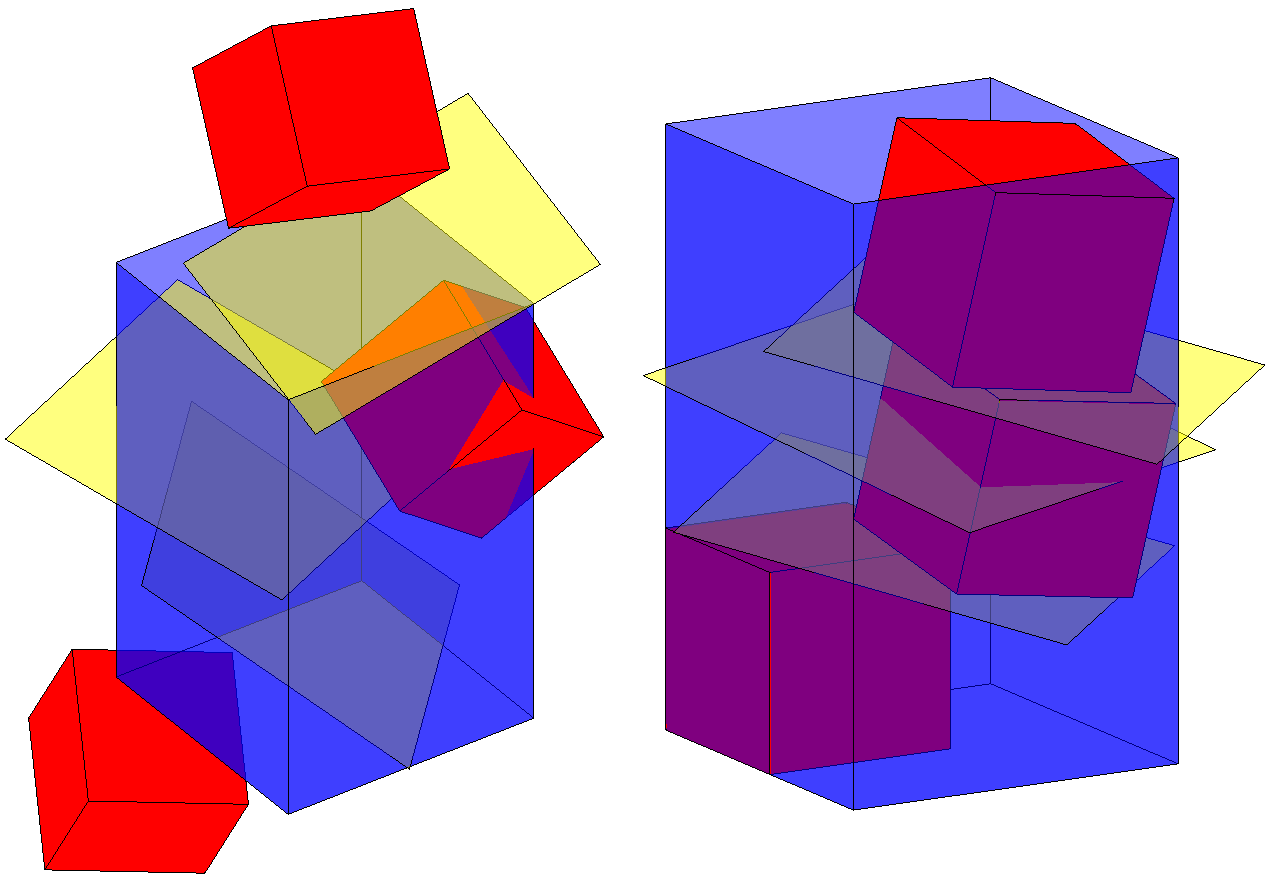
\includegraphics[width=.8\linewidth]{3cubes.png}
  \caption{Problem of stacking 3 red cubes in a blue box, separating each pair of cubes by a yellow plane. Initial (left) and final (right) configurations.}
\label{fig:cubes}
\end{figure}

There is one plane for each pair of cubes, so, $n(n-1)/2$ planes.
Thus the search manifold is:
\begin{equation}
  \mathcal{M} = {\left( \mathbb{R}^3\times SO(3) \right)}^n \times {\left( \mathbb{R} \times S^2 \right)}^{\frac{n(n-1)}{2}} \nonumber
\end{equation}
The problem contains 5 constraints of dimension 8 per cube to fit them in the box and $n(n-1)/2$ constraints of dimension 16 to avoid the interpenetration of cubes.
We have a problem of dimension $4.5n+1.5n^2$ with $32n+8n^2$ constraints.

In order to compare the resolution with and without the use of manifolds, we also formulate this problem over $\mathbb{R}^n$.
To do so, each variable on $SO(3)$ is replaced by a variable on $\mathbb{R}^4$, while each variable on $S^2$ is replaced by one on $\mathbb{R}^3$.
In both cases, a norm-1 constraint on the variable is added to the problem to force those variables on the manifolds.
This results in a problem on
\begin{equation}
  \mathcal{M}={\left( \mathbb{R}^3\times \mathbb{R}^4 \right)}^n \times {\left( \mathbb{R} \times \mathbb{R}^3 \right)}^{\frac{n(n-1)}{2}} = \mathbb{R}^{5n+2n^2} \nonumber
\end{equation}
that is a problem of dimension $5n+2n^2$ with $32.5n+8.5n^2$ constraints, which is $\frac{n(n+1)}{2}$ more variables and constraints than with the manifold formulation.

We solve these two problems for different numbers of cubes and compare the results in terms of number of iterations before convergence, convergence time, and time spent per iterations.
In each resolution, both problems (Real Space and Manifold formulations) are initialized with the same randomized initial guess.
The resolutions with {\tt PGSolver} are set up with the same set of parameters, and the ones with the CFSQP solver uses its default parameters.
The initial positions of the cubes are chosen randomly, and each plane is initialized at a position between the two cubes it separates.
We display the results of these tests in~\Figref{fig:timings-cubes}.
\begin{figure}[htpb]
  \centering
  % This file was created by matlab2tikz.
%
%The latest updates can be retrieved from
%  http://www.mathworks.com/matlabcentral/fileexchange/22022-matlab2tikz-matlab2tikz
%where you can also make suggestions and rate matlab2tikz.
%
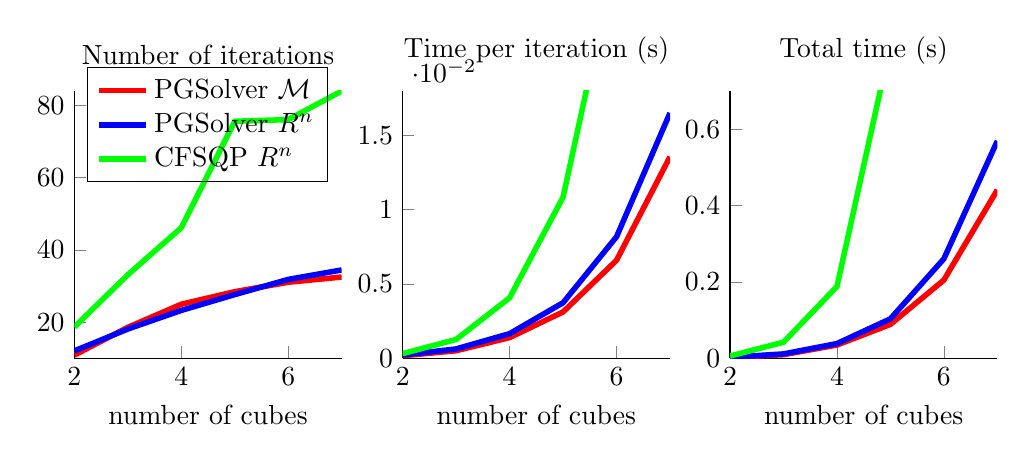
\begin{tikzpicture}
\newcommand{\figSize}{.28\linewidth}
\begin{axis}[%
width=\figSize,
height=\figSize,
at={(2.595in,0.512in)},
scale only axis,
every outer x axis line/.append style={black},
every x tick label/.append style={font=\color{black}},
xmin=2,
xmax=7,
xlabel={number of cubes},
every outer y axis line/.append style={black},
every y tick label/.append style={font=\color{black}},
ymin=10,
ymax=84,
%ylabel={Number of iterations},
axis background/.style={fill=white},
title={Number of iterations},
axis x line*=bottom,
axis y line*=left,
legend style={at={(0.047,0.658)},anchor=south west,legend cell align=left,align=left,fill=none}
]
\addplot [color=red,line width=2pt,solid]
  table[row sep=crcr]{%
2	10.87\\
3	18.5633\\
4	24.9633\\
5	28.4333\\
6	31.0467\\
7	32.4933\\
};
\addlegendentry{PGSolver $\mathcal{M}$};

\addplot [color=blue,line width=2pt,solid]
  table[row sep=crcr]{%
2	12.0467\\
3	18.0967\\
4	23.25\\
5	27.6267\\
6	31.8333\\
7	34.45\\
};
\addlegendentry{PGSolver $\mathbb{R}^n$};

\addplot [color=green,line width=2pt,solid]
  table[row sep=crcr]{%
2	18.6533\\
3	33.1233\\
4	46.14\\
5	75.61\\
6	76.0733\\
7	83.9733\\
};
\addlegendentry{CFSQP $\mathbb{R}^n$};

\end{axis}

\begin{axis}[%
width=\figSize,
height=\figSize,
at={(\figSize + 2.9in ,0.512in)},
scale only axis,
every outer x axis line/.append style={black},
every x tick label/.append style={font=\color{black}},
xmin=2,
xmax=7,
xlabel={number of cubes},
every outer y axis line/.append style={black},
every y tick label/.append style={font=\color{black}},
ymin=0,
ymax=0.018,
%ylabel={Time per iteration (s)},
axis background/.style={fill=white},
title={Time per iteration (s)},
axis x line*=bottom,
axis y line*=left
]
\addplot [color=red,line width=2pt,solid,forget plot]
  table[row sep=crcr]{%
2	0.000169146\\
3	0.00050932\\
4	0.00139202\\
5	0.00312059\\
6	0.00659808\\
7	0.0135693\\
};
\addplot [color=blue,line width=2pt,solid,forget plot]
  table[row sep=crcr]{%
2	0.000218966\\
3	0.000629589\\
4	0.00165723\\
5	0.00374097\\
6	0.00818339\\
7	0.016517\\
};
\addplot [color=green,line width=2pt,solid,forget plot]
  table[row sep=crcr]{%
2	0.000312294\\
3	0.00127155\\
4	0.00407225\\
5	0.0108545\\
6	0.0273492\\
7	0.0461626\\
};
\end{axis}

\begin{axis}[%
width=\figSize,
height=\figSize,
at={(2*\figSize + 3.2in,0.512in)},
scale only axis,
every outer x axis line/.append style={black},
every x tick label/.append style={font=\color{black}},
xmin=2,
xmax=7,
xlabel={number of cubes},
every outer y axis line/.append style={black},
every y tick label/.append style={font=\color{black}},
ymin=0,
ymax=0.7,
%ylabel={Total time (s)},
axis background/.style={fill=white},
title={Total time (s)},
axis x line*=bottom,
axis y line*=left
]
\addplot [color=red,line width=2pt,solid,forget plot]
  table[row sep=crcr]{%
2	0.00183861702\\
3	0.009454659956\\
4	0.034749412866\\
5	0.088728671647\\
6	0.204848610336\\
7	0.44091133569\\
};
\addplot [color=blue,line width=2pt,solid,forget plot]
  table[row sep=crcr]{%
2	0.0026378177122\\
3	0.0113934832563\\
4	0.0385305975\\
5	0.103350655899\\
6	0.260504308887\\
7	0.56901065\\
};
\addplot [color=green,line width=2pt,solid,forget plot]
  table[row sep=crcr]{%
2	0.00582531\\
3	0.04211793\\
4	0.18789362\\
5	0.82070874\\
6	2.0805439 \\
7	3.87642586\\
};
\end{axis}
\end{tikzpicture}%

  \caption{Comparison of resolutions with and without using manifolds with $\mu=10^{-8}$. Red represents the results with {\tt PGSolver} on the manifold formulation, blue on Real Space formulation and green with CFSQP on Real Space formulation.}
\label{fig:timings-cubes}
\end{figure}

With 300 resolutions per case, approximately $98\%$ converged when using a manifold formulation versus $99.5\%$ with a non-manifold formulation with {\tt PGSolver}, whereas the success rates of CFSQP drop incrementally from $100\%$ for 2 cubes to $70\%$ for 7 cubes.
Concerning the resolutions with {\tt PGSolver}, we observe that the numbers of iterations are sensibly similar for the two types of resolutions, but the time spent per iteration is consistently smaller in the case of a resolution with manifolds, which is in agreement with our expectations and subsequently, the convergence time is consistently shorter for the formulation with manifolds.
The resolutions with CFSQP take up to 4 times more iterations and each iteration is on average 3 times longer than with {\tt PGSolver}.
Which results in resolutions with {\tt PGSolver} on manifold formulation being on average 7 times faster than with CFSQP on real-space formulation for this specific type of problem.

During our experimentations, we noticed that the regularization applied on the Hessian of the problem plays an important role in the convergence speed.
In particular, the minimum value for the diagonal terms $\mu$ is important.
We observed that for values of $\mu$ between $10^{-8}$ and $10^{-2}$, the behaviors of both resolutions are quite consistent (the influence of $\mu$ is small in that span), with the best results observed for $10^{-8}$ (presented in~\Figref{fig:timings-cubes}), and the formulation with manifolds is consistently faster than the one without manifolds.
Values outside of that span tend to degrade both resolutions.
Too high values tend to damp the Hessian, which translates into bigger numbers of iterations.
Too small values make the hessian closer to being rank deficient, in that case, we observe larger numbers of internal iterations of the QP solver, which translates into longer times per iteration.

This study shows that on a simple example that makes heavy use of non-Euclidean manifolds, solving a problem on non-Euclidean manifolds with optimization on manifolds not only allows the user to profit of a simpler and more intuitive formulation of the problem but also outperforms the classical approach.
And for this specific problem, {\tt PGSolver} clearly outperforms CFSQP in term of success rates as well as convergence speed.


\section{Evaluation of the Posture Generation}
\label{sec:evaluation_of_the_posture_generation}

In an effort to evaluate the performances of our posture generator framework and solver on manifolds, we devised a campaign of tests in which we solve problems that are known to be feasible and compare the success rates and computation times of different resolution approaches for different types of problems.
We always search viable solutions, where the joint and torque limits are respected, collisions are avoided and static stability is guaranteed.
To generate problems that are known to be feasible, we start by computing the pose of 4 frames that the robot can reach simultaneously with its right foot, left foot, right gripper and left gripper, by querying the Direct Kinematics algorithm for a random configuration $q_\text{rand}$ of the robot that is within its joint limits.
Given those 4 frames, we can create a posture generation problem where the robot has to reach those frames with its end-effectors while respecting its viability constraints.
In particular, we require the contacts on the foot to be fixed unilateral friction contacts (with the forces in the friction cones) and the contacts on the hands to be fixed bilateral contacts (where the forces can be in applied in any direction).
If feasible, this problem can easily be solved by providing as initial guess the configuration $q_\text{rand}$.
If a solution $q^*$ is found, the problem is deemed feasible and is recorded for further use.

Using this process, we compute three types of problems with different sets of constraints:
\begin{itemize}
  \item 2 Contacts: only the foot are in contact, the hands are free of constraints.
  \item 3 Contacts: both foot and the right gripper are in contact, the left hand is free.
  \item 4 Contacts: both foot and hands are in contact.
\end{itemize}

%In addition to evaluating our solver, we want to evaluate the efficiency of our posture generator.
%We propose to study its ability to find a solution to problems that are known to be feasible.

%First, we generate a list of feasible problems.
%To do so, we set the HRP-2 Kai robot in a random configuration $q_\text{rand}$ within its joint limits and record the 3D poses of its end-effectors' frames: at the tip of its grippers and below its foot,we denote them $F_\text{rightGripper}$, $F_\text{leftGripper}$, $F_\text{rightFoot}$, $F_\text{leftFoot}$.
%Then we generate a problem with the constraints that both grippers are in fixed bilateral contact (forces can be applied in any direction) with their associated frames $F_\text{rightGripper}$ and $F_\text{leftGripper}$, while the feet are in unilateral frictional contact (forces in friction cones) with their associated frames $F_\text{rightFoot}$ and $F_\text{leftFoot}$ and the stability, torque limits, and auto-collision avoidance constraints must be respected.
%We solve those problems starting from a configuration close to the solution to estimate their feasibility.
%To make the resolution easier, we initialize the robot's configuration variable to $q_\text{rand}$, which is a solution to the geometric part of the problem.
%If a solution is found, the problem is feasible and is recorded for further use.

%We generate feasible problems by setting a HRP-2 Kai robot's in a random configuration variable $q_\text{rand}$ within its joint limits and recording the poses of its end-effectors' frames: at the tip of its grippers and below its foot,we denote them $F_\text{rightGripper}$, $F_\text{leftGripper}$, $F_\text{rightFoot}$, $F_\text{leftFoot}$.
%Then we check whether that configuration violates the auto-collision constraints, if it does, it is discarded and the process is restarted with another random configuration.

%Once a collision free configuration is found, we generate a problem with the constraints that both gripper are in fixed bilateral contact (forces can be applied in any direction) with their associated frames $F_\text{rightGripper}$ and $F_\text{leftGripper}$, while the foot are in unilateral contact (forces in friction cones) with their associated frames $F_\text{rightFoot}$ and $F_\text{leftFoot}$ and the stability and torque limits must be respected.
%To help the resolution, we initialize the robot's configuration variable to $q_\text{rand}$, which is a solution to the geometric part of the problem.
%If a solution is found, the problem is known to be feasible and recorded for further use.

Some initial testings where we solved the recorded problems with 4 contacts with the half-sitting configuration $q_\text{half-sitting}$ as initial guess showed that a solution is found for only 35\% of the problems.
This is not a surprising result, as the configuration to reach is very far from the initial posture.
We noticed that most of the randomly generated configurations put the robot in a very twisted posture that seems difficult to reach for the optimization algorithm when starting from the half-sitting configuration.

%We evaluate the performance of our posture generator by solving the recorded problems, starting from the half-sitting configuration $q_\text{half-sitting}$ of the robot.
%This approach tests the ability to find a feasible posture when starting from a configuration far from the solution.
%Since there is no cost function, the optimization algorithm is exited as soon as the restoration phase terminates.
%The resolution is successful for approximately 35\% of the problems.
%Which is not surprising, as the configuration to reach is very far from the initial posture.
%We noticed that most of the randomly generated configurations put the robot in a very twisted posture that seems difficult to reach for the optimization algorithm when starting from the half-sitting configuration.

We computed another set of feasible problems in which the value of $q_\text{rand}$ is taken closer to the half-sitting, by taking the average between a random configuration and the half-sitting:
\begin{equation}
  q_\text{rand} \leftarrow \frac{q_\text{rand}+q_\text{half-sitting}}{2}
\end{equation}
%We generate a set of feasible problems from those configurations.
%In that case, a solution is found in 85\% of the tests.
The resolution of those feasible problems showed a rate of success of 85\%.
This implies that the initial guess and its distance from the solution, which we coin the \emph{initial distance}, have a crucial importance in the resolution of posture generation problems.
The initial distance for a problem where $q_0$ is the initial guess and $q^*$ is a solution, is defined as: $d=\|q_0-q^*\|^2$.

%The topology of the problem to solve is also an important factor of the resolution, thus, we generated several sets of feasible problems with different numbers of contact constraints.
%In the first set, contact constraints are only imposed on the two feet of the robot, we denote this set `2 Contacts'.
%In the secont set, contact constraints are imposed on the two feet and the right hand of the robot, we denote this set `3 Contacts'.
%And the last set is the one described previously where contact constraints are imposed on both feet and hands, we denote it `4 Contacts'.
%We study the influence of the initial distance on each of those sets separately.

We propose to evaluate the effect of the initial distance on the success rate and on the convergence time of the posture generator.
In this case, each feasible problem is solved several times, with a value of the initial guess increasingly closer to the solution.
Given a randomly chosen initial guess $q_0$, and $q^*$ being the known solution of the problem, we solve the problem starting from a configuration $q_0^{n\%}$ defined as:
\begin{equation}
  q_0^{n\%} = n q_0 + (1-n)q^*
\end{equation}
With $n$ taking successively the values $1.0$, $0.8$, $0.6$, $0.4$,and $0.2$.
After aggregating the results, we are able to estimate the influence of the initial distance on the success rate and convergence time of the optimization.
During all our work with our solver, we observed that the choice of Hessian approximation method has a substantial effect on the resolution.
We take here the opportunity to assess this observation by solving series of problems with the solver using different Hessian update methods.
As we explained in Chapter~\ref{chapter:optimization_on_noneuclidean_manifolds}, the Hessian can be updated as a whole, or individually, in which case a list of Hessians approximating each constraint's second-order derivative is maintained and combined in the global Hessian matrix.
We compare the results obtained with the three update methods that are BFGS, BFGS with self-scaling and SR1 and using whole or individual updates for each of them.
We gather those results after solving 250 different posture generation problems, 5 times each, starting increasingly close from the solution.
We sample the range of initial distances into 20 segments of the same length and report the average results on each segment as a data point in~\Figref{fig:evalPG}.
\begin{figure}[htb]
\centering
  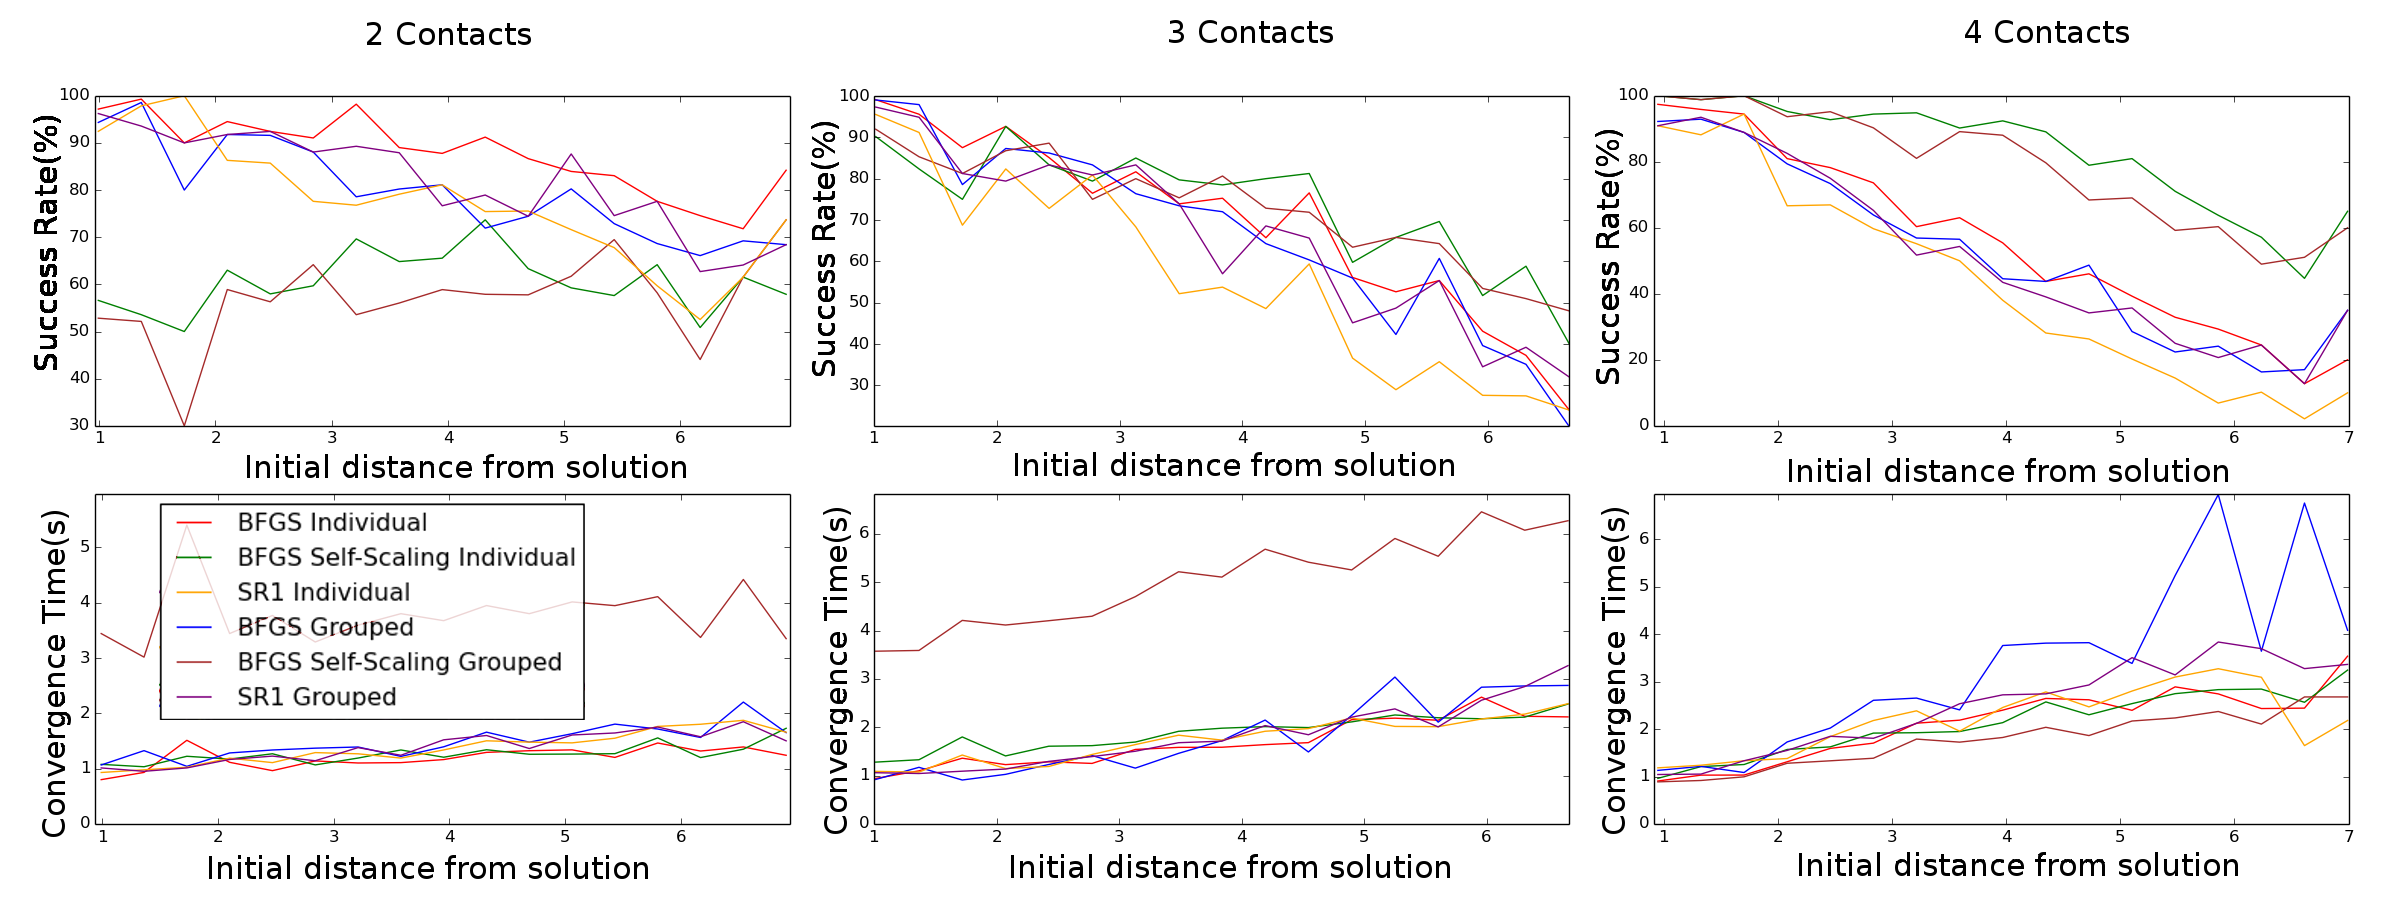
\includegraphics[width=\linewidth]{evalPG/resWithSR1Grouped.png}
  \caption{Comparison of rate of success and convergence times of the posture generation problem resolution with respect to the distance between initial guess and solution for sets of feasible problems with 2, 3 and 4 contact constraints and for different choices of Hessian update methods.}
\label{fig:evalPG}
\end{figure}

The results obtained show that there is not one Hessian update method that is much better than all others in every case.
The BFGS and SR1 approaches with individual or grouped Hessians present similar and consistent behaviors on the 3 types of problems.
The BFGS with self-scaling update is quite inconsistent, as it shows the best success rates and convergence speeds on problems with 4 contact constraints, but the worst ones for problems with 2, and on problems with 3 contacts, the individual update fairs correctly while the grouped one has the worst computation times.
%We observed that those slow convergence times were due to high numbers of iterations and not to high computation times per iteration.
%Whereas the BFGS with and without self

This experiment shows that the closer the initial guess is to the solution, the more likely the solver is to converge to a solution and it gives us a quantitative estimate of the expected success rate and convergence times with respect to the initial distance.

Aside from the BFGS with self-scaling methods, all others usually reach convergence in a few seconds, taking longer when starting further from the solution.
On average, a solution is found faster for problems with only 2 contacts, within 2 seconds, problems with 3 contacts take a little longer, up to 3 seconds, and problems with 4 contacts are the longest to solve, taking up to 4 seconds.

Although those computation times are long, and make it inconvenient to compute large numbers of postures, as is often done in contact planning, they remain of the same order of magnitude as the ones reported in~\cite{brossette:RAM:2013}, \cite{escande:iros:2006}, \cite{bouyarmane2011autonomous} and \cite{hauser:ijrr:2008}, that were all based on off-the-shelf solvers, while we use an open solver that we developed and are able to modify or even specialize.

It would be interesting to run more tests like those to study the influence of the different solver options and find optimal strategies to set the solver's option to solve posture generation problems.
Perhaps choosing automatically the update method and other options based on the structure of the problem at hand would allow increasing the general performance of our posture generator.
%An initial study of the problem to solve, followed by an automatic tuning of the solver seems like a promising idea to improve the posture generator's performances.
%One could for example choose an initial guess amongst a database based on the structure of the problem.
%It would also be possible to take into account the very specific structure of a robot in the resolution algorithm.

\FloatBarrier
\section{Application to Inertial Parameters Identification}
\label{sec:inertial_parameters}

Although it was developed with the idea of solving posture generation problems, our solver and the formulation on manifolds can be used for different types of problems.
In this section, we present an application of our optimization algorithm to solve a problem of inertial parameters identification that was published in~\cite{traversaro:iros:2016}.

\subsection{Physical Consistency of Inertial Parameters}
\label{sub:physical_consistency_of_inertial_parameters}

The dynamics of a rigid body is completely defined by its mass distribution:
\begin{equation}
  \rho(.):\mathbb{R}^3 \mapsto\mathbb{R}_{\geq 0}
\end{equation}
That function defines the density of a rigid body in the 3D space, it is strictly positive on points that belong to the rigid body and null everywhere else.
The complete dynamics of a rigid body can be captured by a set of parameters $\pi\in\mathbb{R}^{10}$ representing its mass $m$, the position of its center of mass $c$ and its 3D inertia matrix $I_B$.
By definition, those parameters are functionals of $\rho(.)$.
The identification of those parameters can in some cases be obtained from the Computer-Aided Design (CAD) model of the body, but it is often necessary to evaluate those parameters experimentally.
Their identification can be done by measuring the body acceleration $A^g$, twist $V$ and the external wrench applied to it $F$ for $N$ different situation and finding $\pi^*$ that minimizes the error in the Newton-Euler equation for those values:
\begin{equation}
\label{eq:classicIdentif}
  \pi^* = \argmin_{\pi\in\mathbb{R}^{10}} \sum_{i=0}^N \|Y(A^g_i,V_i)\pi -F_i\|^2
\end{equation}
Where $Y(A^g_i,V_i)$ is a matrix representing the inertial effects in the Newton-Euler equation.
To take into account the physical properties of the inertial parameters, the \emph{physical consistency} constraint is traditionally used, it enforces that the mass and inertia matrix are respectively positive and positive definite.
In~\cite{traversaro:iros:2016}, we prove that the \emph{physical consistency} constraint is not enough to ensure that there exists a mass distribution for a given set of inertial parameters, thus, we propose an alternate formulation that we call \emph{full physical consistency} that ensures it.
In this novel formulation, the inertial parameters are parametrized by an element $\theta \in \mathfrak{P} = \mathbb{R}_{\ge 0} \times \mathbb{R}^3 \times  SO(3) \times \mathbb{R}_{\ge 0}^3$ and the \emph{full physical consistency} in ensured.
In particular the components of $\theta$ are:
\begin{itemize}
    \item $m \in \mathbb{R}_{\ge 0}$ the mass of the body
    \item $c \in \mathbb{R}^3$ the center of mass of the body
    \item $Q \in SO(3)$ the rotation matrix between the body frame and the frame of principal axes at the center of mass
    \item $L \in \mathbb{R}_{\ge 0}^3$ the second central moment of mass along the principal axes
\end{itemize}
And we devise a functional $\pi_p(\theta):\mathfrak{P}\mapsto\mathbb{R}^{10}$ that maps this new parametrization to the corresponding inertial parameters.
However, the optimization variable now lives on a non-Euclidean manifold, because $\mathfrak{P}$ includes $SO(3)$.
Thus, we propose to solve that problem with our solver on manifolds.

%\subsection{Physical Consistency of Inertial Parameters}
%\label{sub:physical_consistency_of_inertial_parameters}

%The dynamics of a rigid body is completely defined by its mass distribution:
%\begin{equation}
  %\rho(.):\mathbb{R}^3 \mapsto\mathbb{R}_{\geq 0}
%\end{equation}
%That function defines the density of a rigid body in the 3D space, it is strictly positive on points that belong to the rigid body and null everywhere else.
%It can be reduced to 10 inertial parameters $\pi\in\mathbb{R}^{10}$ to describe the dynamics of the rigid body~\cite{hollerbach2008}.
%%which is itself completely described by 10 inertial parameters~\cite{hollerbach2008}.
%%The dynamics of a rigid body is completely defined by its mass distribution, which is itself completely described by 10 inertial parameters~\cite{hollerbach2008}.
%We denote $\text{vech}(.)$ the serialization operation on symmetric matrices.
%\begin{equation}
  %\pi = \begin{bmatrix}
    %m \\
    %mc \\
    %\text{vech}(I_B)
  %\end{bmatrix}
%\end{equation}
%\begin{itemize}
  %\item $m\in\mathbb{R}$ is the mass of the rigid body
  %\item $\hat{c}$ denotes the skew-symmetric matrix associated with $c\in\mathbb{R}^3$, the position of the center of mass of the rigid body
  %\item $I_B\in\mathbb{R}^{3\times 3}$ is its 3D inertia matrix
%\end{itemize}

%%Those parameters are defined as functionals of the mass distribution of the rigid body:
%%\begin{equation}
  %%\rho(.):\mathbb{R}^3 \mapsto\mathbb{R}_{\geq 0}
%%\end{equation}
%%That function defines the density of a rigid body in the 3D space, is is null outside of the body and strictly positive inside it.

%By definition, the inertial parameters are functionals of the mass distribution $\rho(.)$, and can be written as $\pi_d:(\mathbb{R}^3\mapsto\mathbb{R})\mapsto\mathbb{R}^{10}$

%%\begin{equation}
  %%\pi_d\ :\
  %%\begin{array}{ccc}
%%(\mathbb{R}^3 \mapsto \mathbb{R}) & \mapsto & \mathbb{R}^{10}\\
%%\rho(.)
   %%& \rightarrow &
  %%\begin{bmatrix}
    %%\iiint\limits_{\mathbb{R}^3} \rho(r) dr \\
    %%\iiint\limits_{\mathbb{R}^3} r \rho(r) dr \\
    %%\operatorname{vech}\left(
    %%\iiint\limits_{\mathbb{R}^3} {\hat{r}}^\top \hat{r} \rho({r}) d{r} \right)
  %%\end{bmatrix}
  %%\end{array}\nonumber%
%%\end{equation}

%\begin{equation}
%\pi_d(\rho(.))
  %=
  %\begin{bmatrix}
    %\iiint\limits_{\mathbb{R}^3} \rho(r) dr \\
    %\iiint\limits_{\mathbb{R}^3} r \rho(r) dr \\
    %\operatorname{vech}\left(
    %\iiint\limits_{\mathbb{R}^3} {\hat{r}}^\top \hat{r} \rho({r}) d{r} \right)
  %\end{bmatrix}
%\end{equation}

%The identification of those parameters can in some cases be obtained from the Computer-Aided Design (CAD) model of the body, but it is often necessary to evaluate those parameters experimentally.
%Their identification can be done by measuring the body acceleration $A^g$, twist $V$ and the external wrench applied to it $F$ for $N$ different situation and finding $\pi^*$ that minimizes the error in the Newton-Euler equation for those values:
%\begin{equation}
%\label{eq:classicIdentif}
  %\pi^* = \argmin_{\pi\in\mathbb{R}^{10}} \|Y(A^g_i,V_i)\pi -F_i\|^2
%\end{equation}
%%Identifying the inertial parameters of a rigid body comes down to finding $\pi$ that minimizes the error in the Newton-Euler equation~\ref{eq:NewtonEuler}.
%Where $Y(A^g,V)$ is such that:
%$$
%Y(A^g,V)\pi = M A^g + V\bar{\times}^*MV
%$$
%M is the spatial inertia matrix:
%\begin{equation}
%M=
  %\begin{bmatrix}
    %m\mathbb{I}_3 & -m\hat{c} \\
    %m\hat{c} & I_B
  %\end{bmatrix}
%\end{equation}
%and $V \bar \times^*$ is the 6D force cross product operator \cite{featherstone:book:2007} that, for $V = \begin{bmatrix} v^\top & \omega^\top \end{bmatrix}^\top \in \mathbb{R}^6$, gives:
%$$
%V \bar \times^*
%=
%\begin{bmatrix}
%\omega^\top & 0_{3\times3} \\
%v^\top      & \omega^\top
%\end{bmatrix}
%$$

%However, this optimization problem~\ref{eq:classicIdentif} does not take into account the physical properties of the inertial parameters.
%For this, the \emph{physical consistency} constraint is introduced~\cite{yoshida1994} and added to the problem:
%\begin{definition}
  %A vector of inertial parameters $\pi\in\mathbb{R}^{10}$ is called \emph{physical consistent} if:
%\begin{equation}
  %\begin{aligned}
    %m(\pi) \geq 0\\
    %I_C(\pi) \succeq 0
  %\end{aligned}
%\end{equation}
%\end{definition}
%Where $I_C(\pi)$ is the 3D inertial matrix at the center of mass.
%Inertial parameters satisfying the \emph{physical consistency} conditions have nice properties ($M$ is invertible), but it is still possible to find some \emph{physical consistent} inertial parameters that cannot be generated by a mass distribution of a rigid body.
%In~\cite{traversaro:iros:2016}, we propose the \emph{full physical consistent} condition that assesses that a vector of inertial parameters can be generated from a physical rigid body.

%\begin{definition}
  %A vector of inertial parameters $\pi\in\mathbb{R}^{10}$ is called \emph{fully physical consistent} if:
  %\begin{equation}
    %\exists\rho(.):\mathbb{R}^3\mapsto\mathbb{R}_{\geq 0}\ \text{s.t.}\ \pi = \pi_d(\rho(.))
  %\end{equation}
%\end{definition}

%We propose a new parametrization of the inertial parameters by an element $\theta \in \mathfrak{P} = \mathbb{R}_{\ge 0} \times \mathbb{R}^3 \times  SO(3) \times \mathbb{R}_{\ge 0}^3$ that ensures the \emph{full physical consistency}. In particular the components of $\theta$ are:
%\begin{itemize}
    %\item $m \in \mathbb{R}_{\ge 0}$ the mass of body
    %\item $c \in \mathbb{R}^3$ the center of mass of the body
    %\item $Q \in SO(3)$ the rotation matrix between the body frame and the frame of principal axis at the center of mass
    %\item $L \in \mathbb{R}_{\ge 0}^3$ the second central moment of mass along the principal axes
%\end{itemize}
%And a function $\pi_p(\theta):\mathfrak{P}\mapsto\mathbb{R}^{10}$ that maps this new parametrization to the corresponding inertial parameters.
%\begin{equation}
  %\label{eq:pip}
  %\pi_p(\theta)
  %=
  %\begin{bmatrix}
    %m(\theta) \\
    %mc(\theta) \\
    %\operatorname{vech}\left(I_B(\theta)\right) \\
  %\end{bmatrix}
  %=
  %\begin{bmatrix}
    %m \\
    %mc \\
    %\operatorname{vech}\left( Q \operatorname{diag}{(\left[\begin{smallmatrix}
    %0 & 1 & 1 \\
    %1 & 0 & 1 \\
    %1 & 1 & 0
    %\end{smallmatrix}\right] L)}  Q^\top - m \hat{c} \hat{c} \right) \\
  %\end{bmatrix} \nonumber
%\end{equation}
%In~\cite{traversaro:iros:2016}, we prove that every $\theta\in\mathfrak{P}$ generates \emph{fully physically consistent} inertial parameters.
%However, the optimization variable now lives on a non-Euclidean manifold, because $\mathfrak{P}$ includes $SO(3)$.
%Thus, we propose to solve that problem with our solver on manifolds.

\subsection{Resolution with optimization on Manifolds}
\label{sub:resolution_with_optimization_on_manifolds}

The formulation of the problem becomes:

\begin{equation}
\begin{aligned}
\label{eq:finalProblem}
    \argmin_{\theta \in \mathbb{R}\times\mathbb{R}^3\times SO(3) \times \mathbb{R}^3} &\ \sum_{i = 1}^N \left\| Y(A^g_i, V_i) \pi(\theta) - F_i \right\|^2 \\
    \mbox{s.t.} &\ m \geq 0,\ L_x \geq 0,\ L_y \geq 0,\ L_z \geq 0
\end{aligned}
\end{equation}

We can solve it with our solver on manifolds.
It has an immediate advantage: we can write directly the problem ~\eqref{eq:finalProblem} without the need to add any parametrization-related constraints.
Because there are fewer variables and fewer constraints, it is also faster to solve.
To check this, we compared the resolution of~\eqref{eq:finalProblem} formulated with each of the three parametrizations of $SO(3)$ available, namely, native $SO(3)$, unit quaternion and rotation matrix.
We solved the three formulations with our PGSolver, and the two last ones with an off-the-shelf solver (CFSQP~\cite{cfsqp:manual}), using the dataset presented in section~\ref{sub:experiments}.
The formulation with native $SO(3)$ was consistently solved faster.
We observed timings around $0.5$s for it, and over $1$s for non-manifold formulations with CFSQP.
The mean time for an iteration was also the lowest with the native formulation (at least $30\%$ lower when compared to all other possibilities).

Working directly with manifolds has also an advantage that we do not leverage here, but could be useful for future work: at each iteration, the variables of the problem represent a \emph{fully physically consistent} set of inertial parameters.
This is not the case with the other formulations we discussed, as the (additional) constraints are guaranteed to be satisfied only at the end of the optimization process.
Having physically meaningful intermediate values can be useful to evaluate additional functions that presuppose it (additional constraints, external monitoring $\ldots$).
It can also be leveraged for real-time applications where only a short time is allocated repeatedly to the inertial identification, so that when the optimization process is stopped after a few iterations, the output is physically valid.

\subsection{Experiments}
\label{sub:experiments}
We ran some experiments with the iCub robot.
It is a full-body humanoid with 53 degrees of freedom \cite{metta2010icub}.
For validating the presented approach, we used the six-axis force/torque (F/T) sensor embedded in iCub's right arm to collect experimental F/T measurements.
We locked the elbow, wrist and hand joints of the arm, simulating the presence of a rigid body directly attached to the F/T sensor, a scenario similar to the one in which an unknown payload needs to be identified \cite{kubus2008line}.

\begin{figure}[htb]
\centering
\begin{overpic}[width=0.68\textwidth,natwidth=1235,natheight=742]{arm3.png}
\put(5,10){FT sensor}
\put(13,13){\vector(1,1){18}}
\put(38,50){Upper arm}
\put(43,49){\vector(0,-1){12}}
\put(65,45){Forearm}
\put(70,44){\vector(-1,-2){7}}
\end{overpic}
\caption{CAD drawing of the iCub arm used in the experiments. The six-axis F/T sensor used for validation is visible in the middle of the upper arm link.}
\label{fig:cadArm}
\end{figure}

We generated five 60 seconds trajectories in which the three shoulder joints were reaching successive random joint positions using minimum-jerk like trajectories.
Each trajectory is decomposed in sub-trajectories to travel between two consecutive random positions in respectively $10$s, $5$s, $2$s, $1$s and $0.5$s (As a result, the trajectories are ordered from the slowest to the fastest).
We played those trajectories on the robot and sampled the F/T sensors and joint encoders outputs at $100$Hz.
%We filtered the joint positions and obtained joint velocities and accelerations using a Savitzky-Golay filtering of order 2 and with a windows size of $499$, $41$, $21$, $9$, $7$ samples.
We used joint positions, velocities and accelerations with the kinematic model of the robot to compute $A^g$ and $V$ of the F/T sensor for each time sample.
%We removed the unknown offset from the F/T measurements using the offset removal technique described in \cite{traversaro2015situ}.
We solved the inertial identification problem~\eqref{eq:classicIdentif} using a classical linear algorithm and the one using the proposed \emph{fully physically consistent} parametrization \eqref{eq:finalProblem} with our solver on manifolds.
We report the identified inertial parameters in Table \ref{table:results}.
It is interesting to highlight that for slow datasets (sub-trajectory times of $10$s or $5$s) the unconstrained optimization problem \eqref{eq:classicIdentif} results in inertial parameters that are not \emph{fully physically consistent}.
In particular, this is due to the low values of angular velocities and acceleration, that do not properly excite the inertial parameters, which are then \emph{numerically not identifiable}.
\begin{figure}
\centering
  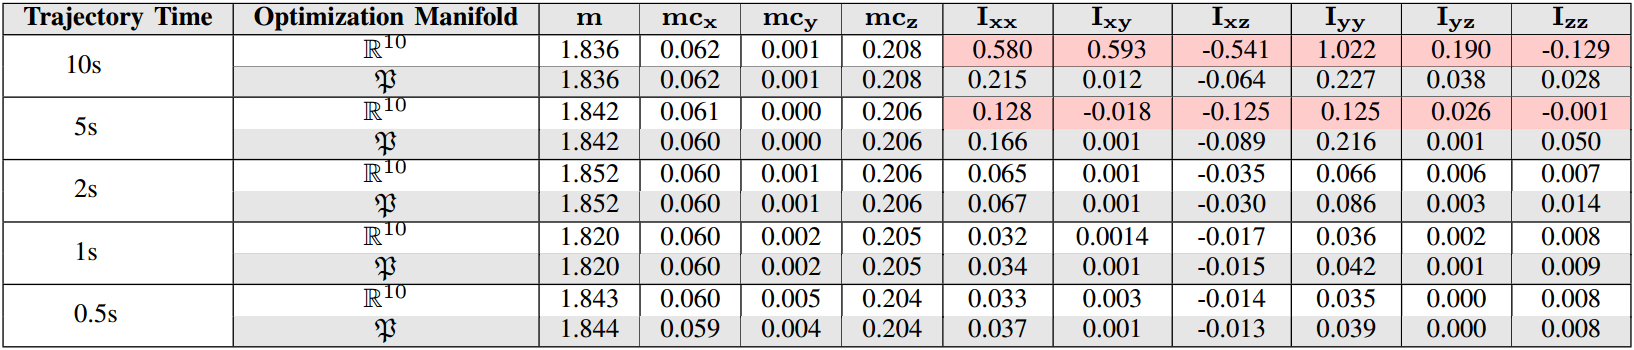
\includegraphics[width=\linewidth]{tableResults.png}
  \caption{Inertial parameters identified with the different datasets and the different optimization problems.
  Inertial parameters identified on $\mathbb{R}^{10}$ optimization manifold that are not \emph{fully physically consistent} are highlighted.
Masses are expressed in $kg$, first moment of masses in $kg.m$, inertia matrix elements in $kg.m^2$.}
\label{table:results}
\end{figure}
\FloatBarrier
The proposed optimization problem clearly cannot identify those parameters anyway, as the identified parameters are an order of magnitude larger than the ones estimated for faster datasets, nevertheless, it always estimates inertial parameters that are \emph{fully physically consistent}.
For faster datasets (sub-trajectory times of $1$s or $0.5$s) the results of the two optimization problems are the same because the high values of angular velocities and accelerations permit to identify all the parameters perfectly.
While this is possible to identify all the inertial parameters of a single rigid body, this is not the case when identifying the inertial parameters of a complex structure such as a humanoid robot, for which both structural \cite{ayusawa2014identifiability} and numerical \cite{pham1991essential} not identifiable parameters exists.
In this later application, the enforcement of \emph{full physical consistency}  will always be necessary to get meaningful results.

\section{Application to contact planning on real-environment}
\label{sec:application_of_contact_planning_on_real_environment}

In this section, we present our approach to generate multi-contact planning scenarios in a sensory acquired environment.
This work was done prior to the development of our posture generator and therefore makes use of a previous version of it that is presented in~\cite{bouyarmane:humanoids:2010}.
Our plan is now to use our Posture Generator in this framework.

Generating isolated postures is not sufficient to make a robot move or achieve tasks in ways similar to humans.
It needs to plan entire motions, with sequences of contact creations and releases, and trajectories in-between.
That's the role of the Multi-Contact Planner (MCP).
The core of the planner consists of the multi-contact search and the posture generator.
The former incrementally builds a tree of contact sets and is presented in~\cite{escande:ras:2013}.
The children of a node are obtained by adding or removing exactly one contact to its set.
At each iteration of the search, the best leaf, according to a potential field, is expanded this way.
The tentative sets of contacts are tested by a posture generator.
Upon success, the contact set is validated, and a new leaf is created.
The goal is written as a set of specific constraints.
A node is a final node if its associated posture generation problem augmented by these constraints remains feasible.
By backtracking from this final node to the initial root node, we obtain a sequence of nodes and thus a sequence of contact sets, that can be executed on the robot by a whole-body controller such as the one based on a quadratic programming (QP) formulation presented in~\cite{bouyarmane:iros:2011}.

The potential field is derived from a crude path, made of a few key postures, that does not take contacts into account.
Such a path is either user-defined or can be the output of a first dedicated planner~\cite{bouyarmane:icra:2009}.

The MCP relies largely on the 3D geometric models of the environment and robotic agents.
In our previous work~\cite{escande:ras:2013,bouyarmane:ar:2012}, the geometric models are provided by the user.
The contact transition for the robot are planned off-line and later executed by the robot assuming exactness of the models and their relative positioning.
We aim at extending our MCP to deal directly with real data acquired by the robot.
Subsequently, we must deal with two kinds of situations:
\begin{enumerate}
  \item the models of the objects in the environment are known: in this case adapting the MCP consists mainly in dealing with recognition, model superposition, and handling uncertainties.
  In brief, once model superposition is achieved, we can use the 3D model for MCP as in~\cite{escande:ras:2013,bouyarmane:ar:2012}, yet some adjustments are needed.
  \item the models of the hurdles and the environment are not known (e.g.\ disaster or outdoor environments, for example, related to the Fukushima disaster that inspired the DARPA Robotic Challenge), MCP is to be achieved in an egocentric way with models built from the robot's embedded sensors.
  This section deals with this case and we describe how the MCP is modified to achieve this goal.
  In a nutshell, we construct planar surfaces from the 3D point clouds data and feed them to the MCP.\@
\end{enumerate}

In robotics, the use of 3D-based vision for recognition and navigation in environments known or partially unknown has first been used on mobile robots, evolving in a flat environment, for example by coupling it with a SLAM system~\cite{whitty:acra:2012}.
Another approach consists in extracting the surfaces from the point cloud, and then link them to the known environment or simply consider them as obstacles to be avoided~\cite{poppinga:iros:2008}.
Since working on raw point clouds is costly because of the high number of data points, this extraction has also been enhanced~\cite{biswas:icra:2012} in order to be run in real-time.
This approach has recently been experimented on a humanoid robot in~\cite{maier:humanoids:2012}, where two methods are combined: the surface extraction from a point cloud, and the voxel-based 3D decomposition of the environment~\cite{nakhaei:humanoids:2008}.
Still, since the robot only navigates in a flat environment, and does not realize manipulation tasks, the surfaces extracted from the 3D point cloud are down projected to a 2D plan, on which are based the navigation and collision avoidance processes.

The use of humanoid robots allows to navigate in more complex environments, some work has been done to make a humanoid robot go down a ramp~\cite{lutz:iros:2012} or climb stairs~\cite{osswald:iros:2012}.
Yet, those methods use laser-based vision rather than point-cloud-based vision, so as to have a precise analysis of a known environment.

In this work, we aim at enabling a robot to analyze and plan a motion into a 3D environment.
Hence, we use the surface extraction of a point cloud to directly have a global picture of the environment and determine the convex planar surfaces that the robot can use to its advantage to progress using the MCP.\@
In our approach to make such an extension, we intentionally seek for technical solutions that minimize changes to be done on the existing MCP software.

\subsection{Building an understandable environment}
\label{sub:building_an_understandable_environment}

Our first concern is to build an environment that our multi-contact planner is able to ``understand'' and that can be extracted from a point cloud scene.

The simplest entity that our planner would be able to deal with and that could correctly describe the robot's environment is a set of convex polygonal planar surfaces.
Therefore, starting from an acquired point cloud, we extract a relevant set of such geometrical entities that will be used as of the surroundings of the robot.

The different steps we follow to create a set of relevant convex polygonal plane surfaces out of an acquired point cloud are the following:

\begin{figure}
\centering
  \includegraphics[width=\linewidth]{complete_pipeline_modified.pdf}
  \caption{Top: flowchart describing the main elements of our algorithm and the type of data that is passed between them. Bottom: the data throughout the process, illustrated in the case of our first experiment.}
\label{fig:full_pipeline}
\end{figure}

The~\Figref{fig:full_pipeline} illustrates the major steps of this point cloud treatment.
We use Willow Garage's Point Cloud Library\footnote{\url{http://pointclouds.org/}} (PCL)~\cite{rusu:icra:2011} extensively for processing the point cloud.

\paragraph{Acquisition of point cloud from an RGB and depth sensor}
The point cloud representing the scene is acquired by an Asus Xtion Pro camera.
The points are defined by their space coordinates and colors.
We do not use the color information except for display purpose.
It may, however, be useful for future developments in matching object models with sensor data and to perform color-based segmentation algorithms.

\paragraph{Filtering}
In order to reduce the computation time and improve the efficiency of our point cloud treatment algorithm, we filter out the points that are too far and use a voxelized grid approach to downsample the remaining point cloud.
This consists of creating a 3D voxel grid over the point cloud and replacing the points in each voxel by their centroid.
(We use this step to reduce the number of points to treat by a factor 5 to 6)

%, it is necessary to reduce the overall size of the data set. We first remove all points further than 5 meters from the camera: such points are not reliable enough and thus a potential source of error for the following steps.
%We know that the data extracted from the Asus Xtion live camera are reliable only for points that are less than 5 meters away from it. Therefore, we eliminate all the
%points that are further than that, since they would only be a source of error and wouldn't carry any valuable information.

%We then downsample the cloud, since it is excessively dense for our purpose. To do so, we use a voxelized grid approach (using the {\tt pcl::VoxelGrid} class): we create a 3D voxel grid over the input point cloud data. Each voxel represents a group of points that are close enough from each other to be represented by a single point that would be their centroid. The centroid is chosen instead of the center of the voxel because it represents the real environment more accurately. Another advantage of this method is that the filter can easily be parametrized by choosing the size of the voxels. Those two steps allow us to greatly reduce the number of points in the data set. Typically, in our experiments, this divides the number of points by a factor 5 to 6.

\paragraph{Region growing segmentation}
We divide a global point cloud scene into clusters of points that belong to the same flat area, by using a region growing algorithm~\cite{poppinga:iros:2008} that regroups the neighboring points that have similar normals into clusters.
%This method is based on the comparison of the angles between the points' normals.
%\note{\sout{This algorithm fits perfectly our needs, because it provides us with a list of sub-clouds (clusters), and each of those represents a flat area of the scene.}}
%It is used right before the planar extraction algorithm in order to obtain an accurate list of points and plane models they represent.

\paragraph{Planar extraction}
For each cluster, we use a plane segmentation to find the plane model that fits the highest number of points.
The outlying points can then be either filtered, or we can try to find another plan to fit them.

\paragraph{Planar projection and hull convex generation}
We extract the convex hull of the projection of each cluster on their respective fitting plan.
%The exact knowledge of all the data points contained in the plane model of a flat area is not necessary for our planning; we can reduce the point cloud to its convex hull without loss of information (except if the surface is concave, but this issue will be tackled in future works). In order to obtain the convex hull of each set of points, we first project every point of the set on its plane model ({\tt pcl::ProjectInliers} class) and then compute the 2D convex hull of the projected set of points ({\tt pcl::ConvexHull} class).
After this step, each plane surface of the scene is represented by a frame composed of the barycentre of the set of points and the convex hull of the surface.

\paragraph{Re-orientation and transfer to the planner}
After re-orienting each frame to get their expression with respect to the world frame, the list of \{frame + convex hull\} can be sent to the planner as a list of contact surface candidates.
%Before sending the previously computed data to the planner, it is necessary to take into account the initial orientation of the camera. Indeed, if the camera was not aiming in a perfectly horizontal direction, then the entire point cloud would be misoriented. Therefore, it is necessary to re-orientate the surfaces before sending them to the planner. To do so, we simply apply a rotation matrix (that is computed from the initial camera orientation) to each of our data set's frame and origin to settle that problem. From there, the transfer of the surfaces to the planner can be done without any specific issue.

%Re-orientation is done as a last step for the sake of performance: obviously we need to re-orient only a few frames, compared to an early re-orientation of the point cloud that would require to apply a transformation on thousands of points.


\subsection{Constraints for surfaces extracted from point clouds}

%Generating postures in which a contact between convex polygonal plane surfaces requires ensuring that the intersection area between the two surfaces is large enough to support the contact.
%One could use the formulation presented in Section~\ref{sec:integration_on_non_inclusive_contacts_in_posture generation}.
%Or more simply a constraint of convex polygon inclusion, which is sufficient for cases such as the ones we study here, where the support surfaces are wide enough for the robot to lean on.

%%We adjusted slightly our planner and posture generator to handle contacts between convex polygonal plane surfaces.
%%The main modification made in the posture generator deals with properly writing the constraints that enforce the inclusion of one surface into another one.
%%In our previous implementation, contacts are searched between rectangular patches attached to the robot body or the environment.

%Such constraint can be written by enforcing that all the points of polygon $S_i$ are located on the left side of all the segments of polygon $S_j$ (provided that the points of $S_j$ are ordered counterclockwise around its normal).
%%For a couple of coplanar surfaces $S_i$, $S_j$ respectively represented by $n$ and $m$ points, this gives rise to a constraint of dimension $n \times m$:
%Given $S_i$ and $S_j$ two surfaces which contours are defined respectively by the sets of points ${p_0, p_1, \ldots, p_n}$ and ${q_0, q_1, \ldots, q_m}$ and $\vec{n}$ a vector normal to $S_i$, the inclusion of $S_i$ in $S_j$ can be written as the following constraint:

%\begin{equation}
%\forall k \in [0, n],\ \forall l \in [0, m],\ \left[\overrightarrow{q_l p_k}\times\overrightarrow{q_l q_{l+1}}\right].\vec{n} \leq 0
%\end{equation}

%\begin{algorithm}
%\caption{Surface inclusion constraints}
%\label{alg:surf_inclusion}
%\begin{algorithmic}
%\State{Let $S_i$ and $S_j$ be two coplanar plane surfaces}
%\State{$S_i = {p_0, p_1, \ldots, p_n}$ and $S_j = {q_0, q_1, \ldots, q_m}$}
%\State{$\vec{N}$ is $S_i$'s normal vector}
%\For{$k = 0 \to n$}
%\For{$l = 0 \to m$}
%\State{Constraint $: \left[\overrightarrow{q_l p_k}\times\overrightarrow{q_l q_{l+1}}\right].\vec{N} \leq 0$}
%\EndFor{}
%\EndFor{}
%\end{algorithmic}
%\end{algorithm}

Once the surfaces are defined, we can choose which ones are suitable for the robot to make contact with.
Using flat contact constraints formulations as described previously.
Although it is not a mandatory step, it allows to reduce the amount of exploration during the planning phase by removing undesired or inappropriate pairs of robot/environment surfaces.
For the time being, this is determined by heuristics that are defined depending on the situation.
If we want the robot to walk on various surfaces, only surfaces that have a normal vector closely aligned with the gravity field would be selected as potential candidates (so as to eliminate the walls and other surfaces on which the robot cannot walk).
Similarly, only surfaces located at a certain height can be considered for hand contact, etc.

For collision avoidance with the environment, we consider each surface generated by our point cloud treatment algorithm as a thin 3D body.
Basically, we extrude each surface by few centimeters in the direction opposite to its normal (provided that this normal is pointing toward the outside of the real body) and create a convex hull surface using {\tt QHull}~\cite{qhull:acm:1996}.

\subsection{Results}
\label{sub:results_pcl_plannif}

We illustrate this approach with two experiments where the HRP-2 robot is required to move $2$m forward.
In both scenarios, this results in climbing on a table (The first one is $71$cm high and the second one is $53$cm high) with the help of various surrounding objects.
The knowledge of the environment and surrounding objects is obtained from a point cloud captured with an RGBD camera.

All the computations of the following experiments are performed on a single thread of an Intel (R) Core (TM) i7--3840QM CPU at 2.80GHz, with 16Go of RAM\@.

\paragraph{Plan 1: irregular stairs}
In this first experiment, the robot has to walk up some irregular stairs made of several random pieces of furniture to reach its goal.
The filtered point cloud was split into 6 plane surfaces.
The whole cloud processing was done in $2.7$ s.
The planner generates a sequence of 11 nodes, some of which are depicted in~\Figref{fig:table-climbing-simulation-stair}{}.
We notice that the robot climbs the stairs one by one without ever putting its two feet on the same step and without any noticeable problem.
In total, 23 nodes were generated and the planning time was $98.4$ s.

\begin{figure}
  \centering
  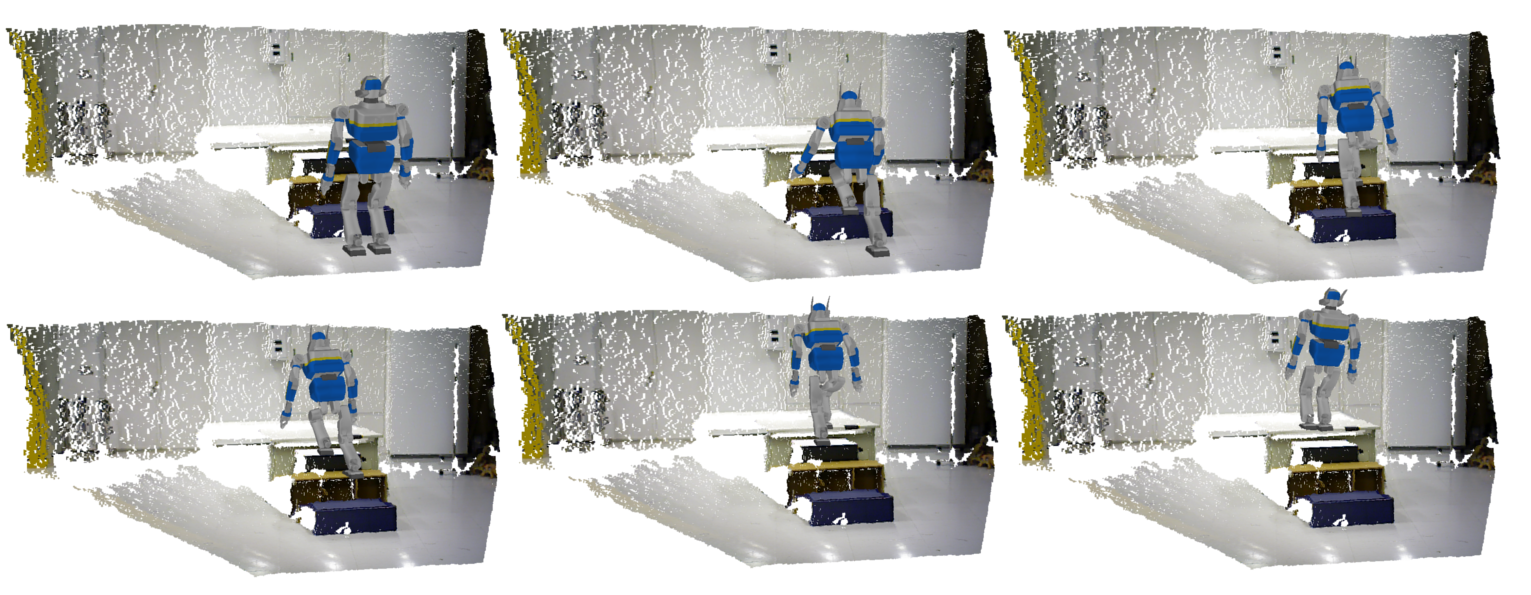
\includegraphics[width=\linewidth]{hrp2stairs.png}
  \caption{Table climbing simulation using irregular stairs. Of the 11 nodes of the path, we depicted the nodes 1, 4, 6, 8, 10 and 11.}
\label{fig:table-climbing-simulation-stair}
\end{figure}

\paragraph{Plan 2: helping motion with the hand}
This second experiment was designed to showcase a more complex plan involving the use of the HRP-2 upper limbs.
In this experiment, we extracted 11 plan surfaces from the point cloud.
The point cloud processing took $2.7$ s.
The planner computation generates a path of 19 nodes, some of which are depicted in~\Figref{fig:crapahut-simulation}{}.
To climb on the table, the robot uses its left arm and walks on an inclined slope before climbing a step at the end of the slope, once again, with the help of its left arm as support.
In total, 40 nodes were generated and the planning time was $122.3$ s.

\begin{figure}
  \centering
  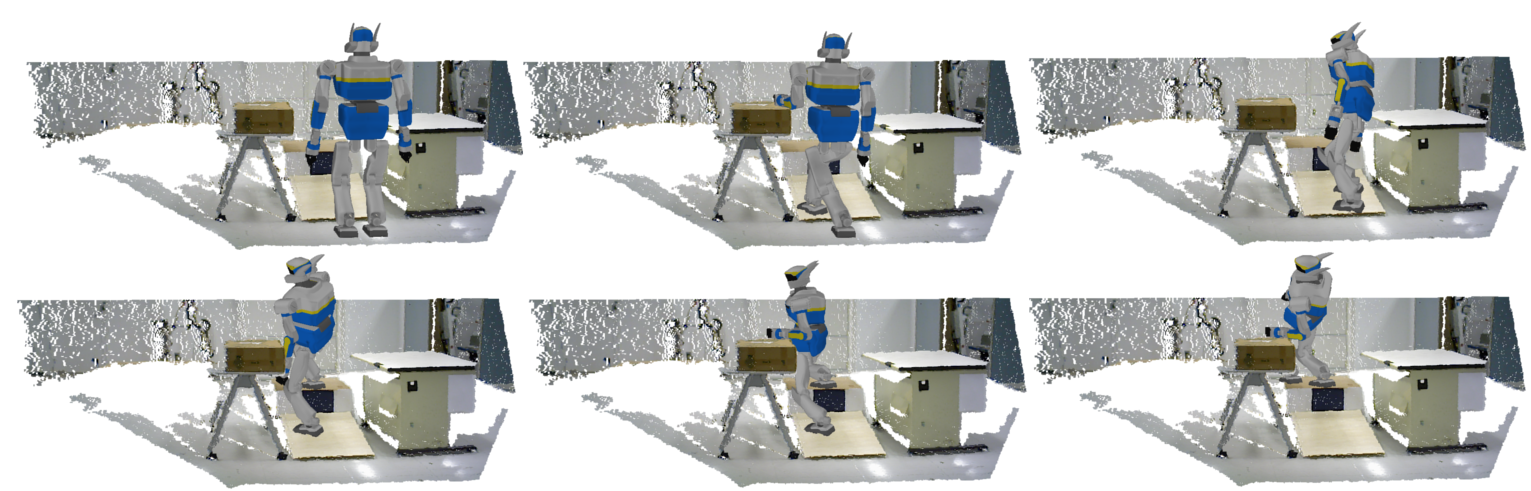
\includegraphics[width=\linewidth]{hrp2slope.png}
  \caption{Slope and step climbing simulation. Of the 19 nodes of the path, we depicted the nodes 1, 7, 12, 15, 17 and 18.}
\label{fig:crapahut-simulation}
\end{figure}

\subsection{Discussion}
\label{sub:discussion_planning_pcl}

This work is a first step toward a fully sensory-perception-based multi-contact planner.
It raises several interesting questions on the way to adapt our MCP\@.

One advantage of our approach is to avoid having to precisely position the robot in the environment prior to the plan execution.
Yet, for now, the positioning is done once and for all with the acquisition of the point cloud, before planning.
When executing the plan, the robot might still deviate from it, for example, a support might move, or a foot might contact a few centimeters away from where it was planned to, or the support might not be at its expected position because of measurement errors in the acquired point cloud.
We thus need to close the loop between the planning and its execution.
To do so, we need robust detection of discrepancies to be made by the robot.
This can be achieved by combining point-cloud-based SLAM with contact sensing.
Once the robot has acquired knowledge of its deviation or of the position error of the support, it has to adapt to it.
This adaptation should not be time-consuming so as to not interrupt the execution for too long.
A slight deviation can be recovered by simply positioning with care the next contacts and the closed-loop multi-contact controller shall work on guarded-motions basis.
However, a bigger deviation might make the next contact stances infeasible.
In this later case, re-planning the next contacts is necessary to go back to the plan.
How many contacts have to be re-planned depends on the context.
In difficult situations, changes in contacts might cascade up to requiring an entire re-planning.
Recognizing the situation should be the task of a local planner that re-plans as few steps as possible.
In case too much contacts must be reprocessed, the re-planning phase can be stopped before it ends and resumed at the next step.

This partial planning approach can also be seen in the context of semi-autonomous motion: an operator gives the overall direction with, for example, a joystick, and the planner reactively finds a sequence of a few contact sets to move as closely as possible in this desired direction.
The operator is thus in charge of preventing the robot from getting stuck while the planner only concentrates on finding the correct contacts over a short time window.

Another question stems from the partial knowledge of the environment: it is not possible to give a guide path as we used to do with the 3D models.
This guide path will necessarily be very crude, either a straight line to the desired position or a plan in a known environment before it was changed (for example in the case of a disaster in a plant).
The planning must then be driven also by the need of getting information about the environment, for example reaching a viewpoint allowing to see parts of the environment that were hidden before, filling empty spaces and possibly adding new supports on-the-fly.
Planning is then only partial since necessary part of the environment might be unknown.

Later on, the discovery of the environment might be improved by the use of other sensors.
One can then imagine having the robot test a contact to ensure a given surface is fit for support or that it is precisely at the position measured by vision.
If the surface is not, this is another kind of discrepancy in the plan that needs to be handled by re-planning.

%We present preliminary results in extending our previous work in multi-contact planning to operate directly on environment that is built on-the-fly from a robot's embedded sensors.
%This first study makes use of depth camera and implemented modules from the PCL which extract planar surfaces that are fed to our MCP\@.
%We intentionally seek for technical implementations that minimize the changes on our existing MCP software and illustrate successful plans generated on the basis of 3D point clouds solely.

The simulation results revealed that our MCP does not require major adjustments to handle egocentric sensory data.
%Of course, this does not mean that we are fully satisfied since our results also suggest additional future work.

Although we choose to treat the case of not having 3D models, we believe that the implementation of an MCP with knowledge of the 3D model is necessary.
For example, even in a disaster situation as in Fukushima nuclear power plants, the inside exploration videos available show that many objects kept their shape and were not totally destroyed (e.g.\ door, stairs, ladders, etc\ldots).
So having their models would then still permit our MCP to rely on 3D models to plan contacts for motion.
PCL provides only partial information, it is then necessary to drive the planner by the mission objective and also a perceptual one (e.g.\ SLAM).
%Of course, our ultimate future plan is to handle uncertainties, control and planning recovery of discrepancies when they occur.

%\section{Examples of postures generation}
%\label{sec:examples_of_postures_generation}

%In this section, we present some scenarios solved with our posture generator and solver.
%\paragraph{Application of a desired force}
%In the context of using a robot to help humans in the construction of an aircraft, we formulate a problem where the HRP-4 robot is required to apply a desired force on a given point of the airplanes structure.
%We denote $f_g$ the target value of the force in direction $\vec{d}$ and $\vec{f_c}$ the actual force at the contact point and the could simply implement the following function $f_{target}(f_c)$ to minimize to get the desired result:
%\begin{equation}
  %f_{target}(f_c) = {\vec{f_c}\cdot\vec{d}-f_g)}^2
%\end{equation}
%In addition to that cost function, the robot needs keep its foot on the ground, its left hand is used to lean on a beam of the structure to allow a longer reach with the right hand that is in contact with the wall.
%Those constraints must be satisfied while respecting the joint and torque limits of the robot, maintaining balance and avoiding auto-collisions.
%The result is depicted in~\Figref{fig:comanoid}
%\begin{figure}
  %\centering
  %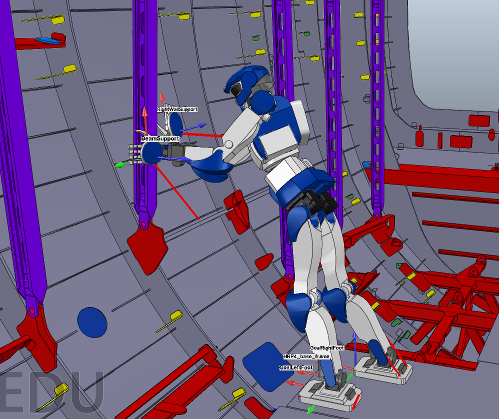
\includegraphics[width=0.6\linewidth]{comanoid.png}
  %\caption{HRP-4 applying a desired force on a contact point with its right hand}
%\label{fig:comanoid}
%\end{figure}

%\paragraph{Generating postures in highly constrained environment}
%In this scenario, the HRP-4 robot is required to evolve in a highly constrained environment, in the sense that many obstacles limit its displacement, and it must avoid collision with them.
%The goal is to real a pannel of circuit breakers (in green on~\Figref{fig:getafe}) to activate them.
%We generated a sequence of steps to reach that panel and then some postures to reach different points of this panel.
%In figure~\ref{fig:getafe}, we show some extracts of this sequence of postures.
%In each of them the two foot are in planar contact with the ground, alternatively bearing forces, while always respecting the joint, torque limits, collision avoidance and stability constraints.
%On the last posture the top left corner of the panel is reached with the tip of the right hand of the robot.
%\begin{figure}
  %\centering
  %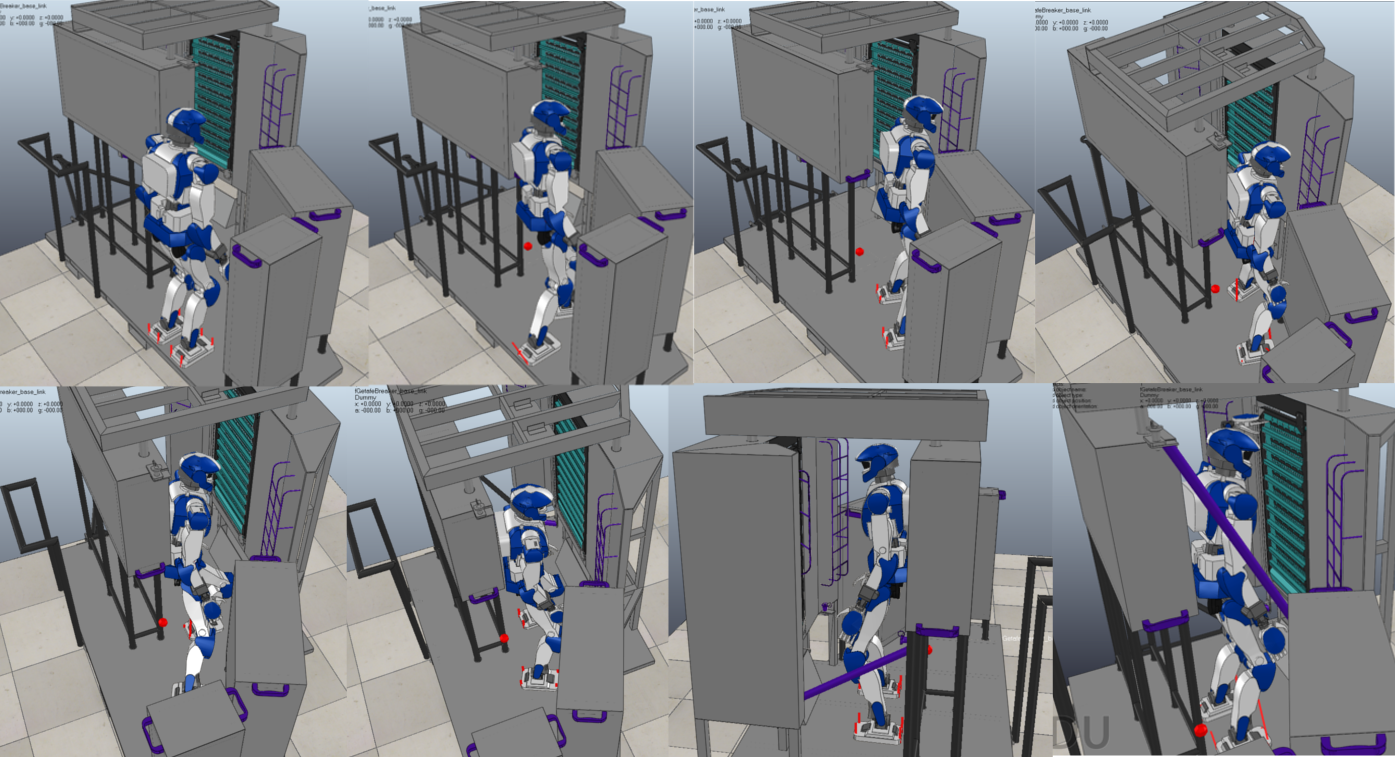
\includegraphics[width=\linewidth]{getafeSequence.png}
  %\caption{Extracts of a sequence of postures with HRP-4 entering a constrained environments to reach a point on a pannel of circuit breakers (in green)}
%\label{fig:getafe}
%\end{figure}


\section{Conclusion}
\label{sec:conclusion_chap_6}

In this section, we presented several evaluations and applications of our solver and posture generator.
We first evaluated the influence of the formulation on manifolds on a problem making heavy usage of them and showed that as expected, this formulation outperforms the classical approach in terms of convergence times.
Then we propose an approach to estimate the success rate of our posture generator with respect to the distance between the initial guess and the solution.
We then present a different application of our solver to the problem of inertial identification of a rigid body.
In which case, working with manifolds ensures the \emph{full physical consistency} of the inertial parameters in any situation and all along the optimization process.
There again, the formulation with manifolds outperforms the classical approach.
We then present an application of posture generation to the problem of planning in a real environment, where we propose a method to segment a sensory acquired environment to allow the generation of postures on it.
Finally, we present some use case scenarios in which our posture generator has been used efficiently.
